\batchmode
\documentclass[twoside]{book}

% Packages required by doxygen
\usepackage{fixltx2e}
\usepackage{calc}
\usepackage{doxygen}
\usepackage[export]{adjustbox} % also loads graphicx
\usepackage{graphicx}
\usepackage[utf8]{inputenc}
\usepackage{makeidx}
\usepackage{multicol}
\usepackage{multirow}
\PassOptionsToPackage{warn}{textcomp}
\usepackage{textcomp}
\usepackage[nointegrals]{wasysym}
\usepackage[table]{xcolor}

% Font selection
\usepackage[T1]{fontenc}
\usepackage[scaled=.90]{helvet}
\usepackage{courier}
\usepackage{amssymb}
\usepackage{sectsty}
\renewcommand{\familydefault}{\sfdefault}
\allsectionsfont{%
  \fontseries{bc}\selectfont%
  \color{darkgray}%
}
\renewcommand{\DoxyLabelFont}{%
  \fontseries{bc}\selectfont%
  \color{darkgray}%
}
\newcommand{\+}{\discretionary{\mbox{\scriptsize$\hookleftarrow$}}{}{}}

% Page & text layout
\usepackage{geometry}
\geometry{%
  a4paper,%
  top=2.5cm,%
  bottom=2.5cm,%
  left=2.5cm,%
  right=2.5cm%
}
\tolerance=750
\hfuzz=15pt
\hbadness=750
\setlength{\emergencystretch}{15pt}
\setlength{\parindent}{0cm}
\setlength{\parskip}{3ex plus 2ex minus 2ex}
\makeatletter
\renewcommand{\paragraph}{%
  \@startsection{paragraph}{4}{0ex}{-1.0ex}{1.0ex}{%
    \normalfont\normalsize\bfseries\SS@parafont%
  }%
}
\renewcommand{\subparagraph}{%
  \@startsection{subparagraph}{5}{0ex}{-1.0ex}{1.0ex}{%
    \normalfont\normalsize\bfseries\SS@subparafont%
  }%
}
\makeatother

% Headers & footers
\usepackage{fancyhdr}
\pagestyle{fancyplain}
\fancyhead[LE]{\fancyplain{}{\bfseries\thepage}}
\fancyhead[CE]{\fancyplain{}{}}
\fancyhead[RE]{\fancyplain{}{\bfseries\leftmark}}
\fancyhead[LO]{\fancyplain{}{\bfseries\rightmark}}
\fancyhead[CO]{\fancyplain{}{}}
\fancyhead[RO]{\fancyplain{}{\bfseries\thepage}}
\fancyfoot[LE]{\fancyplain{}{}}
\fancyfoot[CE]{\fancyplain{}{}}
\fancyfoot[RE]{\fancyplain{}{\bfseries\scriptsize Generated by Doxygen }}
\fancyfoot[LO]{\fancyplain{}{\bfseries\scriptsize Generated by Doxygen }}
\fancyfoot[CO]{\fancyplain{}{}}
\fancyfoot[RO]{\fancyplain{}{}}
\renewcommand{\footrulewidth}{0.4pt}
\renewcommand{\chaptermark}[1]{%
  \markboth{#1}{}%
}
\renewcommand{\sectionmark}[1]{%
  \markright{\thesection\ #1}%
}

% Indices & bibliography
\usepackage{natbib}
\usepackage[titles]{tocloft}
\setcounter{tocdepth}{3}
\setcounter{secnumdepth}{5}
\makeindex

% Hyperlinks (required, but should be loaded last)
\usepackage{ifpdf}
\ifpdf
  \usepackage[pdftex,pagebackref=true]{hyperref}
\else
  \usepackage[ps2pdf,pagebackref=true]{hyperref}
\fi
\hypersetup{%
  colorlinks=true,%
  linkcolor=blue,%
  citecolor=blue,%
  unicode%
}

% Custom commands
\newcommand{\clearemptydoublepage}{%
  \newpage{\pagestyle{empty}\cleardoublepage}%
}

\usepackage{caption}
\captionsetup{labelsep=space,justification=centering,font={bf},singlelinecheck=off,skip=4pt,position=top}

%===== C O N T E N T S =====

\begin{document}

% Titlepage & ToC
\hypersetup{pageanchor=false,
             bookmarksnumbered=true
            }
\pagenumbering{alph}
\pagenumbering{arabic}
\hypersetup{pageanchor=true}

%--- Begin generated contents ---
\chapter{Demo problem\+: Large-\/amplitude shear deformation of a 3D elastic solid}
\label{index}\hypertarget{index}{}\hypertarget{index_q}{}\section{A few quick questions...}\label{index_q}
Since {\ttfamily oomph-\/lib} is developed as open-\/source software, any evidence that the code is being downloaded and used is very helpful for us as it helps to justify our continued work on this project.

We would therefore be extremely grateful if you could provide the information requested in the form below. Pressing the \char`\"{}submit\char`\"{} button will get you to the actual download page.

{\bfseries Note\+:} 
\begin{DoxyItemize}
\item All information will be treated as confidential. 
\item If you provide your email address and check the appropriate box we will add you to our mailing list to inform you of upgrades and bug fixes to the code. Rest assured that the mailing list is {\bfseries very low volume} -- we have better things to do than to bombard you with email. 
\item If you still feel reluctant to provide any of the information requested, feel free to enter some dummy input. The form will check that {\bfseries some} information has been entered but entering your name as \char`\"{}\+Joe Cool\char`\"{} is perfectly acceptable -- this is to discourage people from not providing the information simply because they are too lazy to type... 
\end{DoxyItemize}



 







 

 \hypertarget{index_pdf}{}\section{P\+D\+F file}\label{index_pdf}
A \href{../latex/refman.pdf}{\tt pdf version} of this document is available. \end{document}

\chapter{Namespace Index}
\section{Namespace List}
Here is a list of all namespaces with brief descriptions\+:\begin{DoxyCompactList}
\item\contentsline{section}{\hyperlink{namespaceGlobal__Physical__Variables}{Global\+\_\+\+Physical\+\_\+\+Variables} \\*Global variables that represent physical properties }{\pageref{namespaceGlobal__Physical__Variables}}{}
\item\contentsline{section}{\hyperlink{namespaceoomph}{oomph} }{\pageref{namespaceoomph}}{}
\item\contentsline{section}{\hyperlink{namespacePhysical__Variables}{Physical\+\_\+\+Variables} \\*Namespace for the solution of 2D linear shell equation }{\pageref{namespacePhysical__Variables}}{}
\end{DoxyCompactList}

\chapter{Hierarchical Index}
\section{Class Hierarchy}
This inheritance list is sorted roughly, but not completely, alphabetically\+:\begin{DoxyCompactList}
\item Problem\begin{DoxyCompactList}
\item \contentsline{section}{Unstructured\+Solid\+Problem$<$ E\+L\+E\+M\+E\+NT $>$}{\pageref{classUnstructuredSolidProblem}}{}
\end{DoxyCompactList}
\end{DoxyCompactList}

\chapter{Class Index}
\section{Class List}
Here are the classes, structs, unions and interfaces with brief descriptions\+:\begin{DoxyCompactList}
\item\contentsline{section}{\hyperlink{classPMLProblem}{P\+M\+L\+Problem$<$ E\+L\+E\+M\+E\+N\+T $>$} }{\pageref{classPMLProblem}}{}
\item\contentsline{section}{\hyperlink{classGlobalParameters_1_1TestPMLMapping}{Global\+Parameters\+::\+Test\+P\+M\+L\+Mapping} }{\pageref{classGlobalParameters_1_1TestPMLMapping}}{}
\end{DoxyCompactList}

\chapter{File Index}
\section{File List}
Here is a list of all files with brief descriptions\+:\begin{DoxyCompactList}
\item\contentsline{section}{\hyperlink{jeffery__orbit_8cc}{jeffery\+\_\+orbit.\+cc} }{\pageref{jeffery__orbit_8cc}}{}
\item\contentsline{section}{\hyperlink{jeffery__orbit_8txt__doxygenified_8h}{jeffery\+\_\+orbit.\+txt\+\_\+doxygenified.\+h} }{\pageref{jeffery__orbit_8txt__doxygenified_8h}}{}
\item\contentsline{section}{\hyperlink{my__taylor__hood__elements_8h}{my\+\_\+taylor\+\_\+hood\+\_\+elements.\+h} }{\pageref{my__taylor__hood__elements_8h}}{}
\end{DoxyCompactList}

\chapter{Namespace Documentation}
\hypertarget{namespaceGlobal__Physical__Variables}{}\section{Global\+\_\+\+Physical\+\_\+\+Variables Namespace Reference}
\label{namespaceGlobal__Physical__Variables}\index{Global\+\_\+\+Physical\+\_\+\+Variables@{Global\+\_\+\+Physical\+\_\+\+Variables}}


Namespace for physical parameters.  


\subsection*{Functions}
\begin{DoxyCompactItemize}
\item 
Vector$<$ double $>$ \hyperlink{namespaceGlobal__Physical__Variables_afae321364975eb56688ad13abc8ed6b7}{Gravity} (2)
\begin{DoxyCompactList}\small\item\em Gravity vector. \end{DoxyCompactList}\item 
void \hyperlink{namespaceGlobal__Physical__Variables_a87da705b8a46bed337cf5dbdd788b87b}{body\+\_\+force} (const double \&time, const Vector$<$ double $>$ \&x, Vector$<$ double $>$ \&result)
\begin{DoxyCompactList}\small\item\em Functional body force. \end{DoxyCompactList}\item 
void \hyperlink{namespaceGlobal__Physical__Variables_a9780d615ae07c4e00a436ab2973b54e6}{zero\+\_\+body\+\_\+force} (const double \&time, const Vector$<$ double $>$ \&x, Vector$<$ double $>$ \&result)
\begin{DoxyCompactList}\small\item\em Zero functional body force. \end{DoxyCompactList}\end{DoxyCompactItemize}
\subsection*{Variables}
\begin{DoxyCompactItemize}
\item 
double \hyperlink{namespaceGlobal__Physical__Variables_ab814e627d2eb5bc50318879d19ab16b9}{Re} =100
\begin{DoxyCompactList}\small\item\em Reynolds number. \end{DoxyCompactList}\item 
double \hyperlink{namespaceGlobal__Physical__Variables_ab1a845a672b4d74b304639a976dc65c6}{Re\+\_\+inv\+Fr} =100
\begin{DoxyCompactList}\small\item\em Reynolds/\+Froude number. \end{DoxyCompactList}\end{DoxyCompactItemize}


\subsection{Detailed Description}
Namespace for physical parameters. 

\subsection{Function Documentation}
\mbox{\Hypertarget{namespaceGlobal__Physical__Variables_a87da705b8a46bed337cf5dbdd788b87b}\label{namespaceGlobal__Physical__Variables_a87da705b8a46bed337cf5dbdd788b87b}} 
\index{Global\+\_\+\+Physical\+\_\+\+Variables@{Global\+\_\+\+Physical\+\_\+\+Variables}!body\+\_\+force@{body\+\_\+force}}
\index{body\+\_\+force@{body\+\_\+force}!Global\+\_\+\+Physical\+\_\+\+Variables@{Global\+\_\+\+Physical\+\_\+\+Variables}}
\subsubsection{\texorpdfstring{body\+\_\+force()}{body\_force()}}
{\footnotesize\ttfamily void Global\+\_\+\+Physical\+\_\+\+Variables\+::body\+\_\+force (\begin{DoxyParamCaption}\item[{const double \&}]{time,  }\item[{const Vector$<$ double $>$ \&}]{x,  }\item[{Vector$<$ double $>$ \&}]{result }\end{DoxyParamCaption})}



Functional body force. 



Definition at line 62 of file circular\+\_\+driven\+\_\+cavity.\+cc.



References Re\+\_\+inv\+Fr.



Referenced by main().

\mbox{\Hypertarget{namespaceGlobal__Physical__Variables_afae321364975eb56688ad13abc8ed6b7}\label{namespaceGlobal__Physical__Variables_afae321364975eb56688ad13abc8ed6b7}} 
\index{Global\+\_\+\+Physical\+\_\+\+Variables@{Global\+\_\+\+Physical\+\_\+\+Variables}!Gravity@{Gravity}}
\index{Gravity@{Gravity}!Global\+\_\+\+Physical\+\_\+\+Variables@{Global\+\_\+\+Physical\+\_\+\+Variables}}
\subsubsection{\texorpdfstring{Gravity()}{Gravity()}}
{\footnotesize\ttfamily Vector$<$double$>$ Global\+\_\+\+Physical\+\_\+\+Variables\+::\+Gravity (\begin{DoxyParamCaption}\item[{2}]{ }\end{DoxyParamCaption})}



Gravity vector. 



Referenced by main(), and Quarter\+Circle\+Driven\+Cavity\+Problem$<$ E\+L\+E\+M\+E\+N\+T $>$\+::\+Quarter\+Circle\+Driven\+Cavity\+Problem().

\mbox{\Hypertarget{namespaceGlobal__Physical__Variables_a9780d615ae07c4e00a436ab2973b54e6}\label{namespaceGlobal__Physical__Variables_a9780d615ae07c4e00a436ab2973b54e6}} 
\index{Global\+\_\+\+Physical\+\_\+\+Variables@{Global\+\_\+\+Physical\+\_\+\+Variables}!zero\+\_\+body\+\_\+force@{zero\+\_\+body\+\_\+force}}
\index{zero\+\_\+body\+\_\+force@{zero\+\_\+body\+\_\+force}!Global\+\_\+\+Physical\+\_\+\+Variables@{Global\+\_\+\+Physical\+\_\+\+Variables}}
\subsubsection{\texorpdfstring{zero\+\_\+body\+\_\+force()}{zero\_body\_force()}}
{\footnotesize\ttfamily void Global\+\_\+\+Physical\+\_\+\+Variables\+::zero\+\_\+body\+\_\+force (\begin{DoxyParamCaption}\item[{const double \&}]{time,  }\item[{const Vector$<$ double $>$ \&}]{x,  }\item[{Vector$<$ double $>$ \&}]{result }\end{DoxyParamCaption})}



Zero functional body force. 



Definition at line 70 of file circular\+\_\+driven\+\_\+cavity.\+cc.



Referenced by main().



\subsection{Variable Documentation}
\mbox{\Hypertarget{namespaceGlobal__Physical__Variables_ab814e627d2eb5bc50318879d19ab16b9}\label{namespaceGlobal__Physical__Variables_ab814e627d2eb5bc50318879d19ab16b9}} 
\index{Global\+\_\+\+Physical\+\_\+\+Variables@{Global\+\_\+\+Physical\+\_\+\+Variables}!Re@{Re}}
\index{Re@{Re}!Global\+\_\+\+Physical\+\_\+\+Variables@{Global\+\_\+\+Physical\+\_\+\+Variables}}
\subsubsection{\texorpdfstring{Re}{Re}}
{\footnotesize\ttfamily double Global\+\_\+\+Physical\+\_\+\+Variables\+::\+Re =100}



Reynolds number. 



Definition at line 53 of file circular\+\_\+driven\+\_\+cavity.\+cc.



Referenced by Quarter\+Circle\+Driven\+Cavity\+Problem$<$ E\+L\+E\+M\+E\+N\+T $>$\+::\+Quarter\+Circle\+Driven\+Cavity\+Problem().

\mbox{\Hypertarget{namespaceGlobal__Physical__Variables_ab1a845a672b4d74b304639a976dc65c6}\label{namespaceGlobal__Physical__Variables_ab1a845a672b4d74b304639a976dc65c6}} 
\index{Global\+\_\+\+Physical\+\_\+\+Variables@{Global\+\_\+\+Physical\+\_\+\+Variables}!Re\+\_\+inv\+Fr@{Re\+\_\+inv\+Fr}}
\index{Re\+\_\+inv\+Fr@{Re\+\_\+inv\+Fr}!Global\+\_\+\+Physical\+\_\+\+Variables@{Global\+\_\+\+Physical\+\_\+\+Variables}}
\subsubsection{\texorpdfstring{Re\+\_\+inv\+Fr}{Re\_invFr}}
{\footnotesize\ttfamily double Global\+\_\+\+Physical\+\_\+\+Variables\+::\+Re\+\_\+inv\+Fr =100}



Reynolds/\+Froude number. 



Definition at line 56 of file circular\+\_\+driven\+\_\+cavity.\+cc.



Referenced by body\+\_\+force(), and Quarter\+Circle\+Driven\+Cavity\+Problem$<$ E\+L\+E\+M\+E\+N\+T $>$\+::\+Quarter\+Circle\+Driven\+Cavity\+Problem().


\chapter{Class Documentation}
\hypertarget{classElasticCubicMesh}{}\section{Elastic\+Cubic\+Mesh$<$ E\+L\+E\+M\+E\+NT $>$ Class Template Reference}
\label{classElasticCubicMesh}\index{Elastic\+Cubic\+Mesh$<$ E\+L\+E\+M\+E\+N\+T $>$@{Elastic\+Cubic\+Mesh$<$ E\+L\+E\+M\+E\+N\+T $>$}}


Simple cubic mesh upgraded to become a solid mesh.  


Inheritance diagram for Elastic\+Cubic\+Mesh$<$ E\+L\+E\+M\+E\+NT $>$\+:\begin{figure}[H]
\begin{center}
\leavevmode
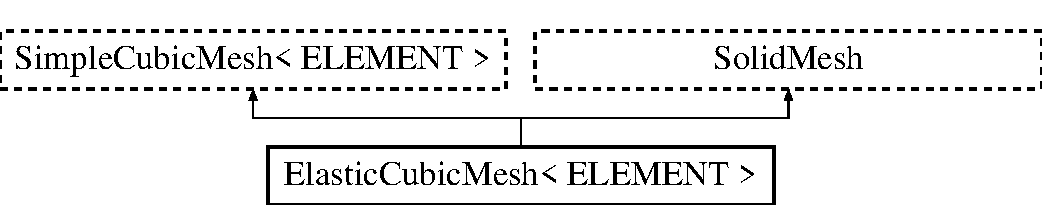
\includegraphics[height=2.000000cm]{classElasticCubicMesh}
\end{center}
\end{figure}
\subsection*{Public Member Functions}
\begin{DoxyCompactItemize}
\item 
\hyperlink{classElasticCubicMesh_aa09317d23e99358728bd81d0c67410a4}{Elastic\+Cubic\+Mesh} (const unsigned \&nx, const unsigned \&ny, const unsigned \&nz, const double \&a, const double \&b, const double \&c, Time\+Stepper $\ast$time\+\_\+stepper\+\_\+pt=\&Mesh\+::\+Default\+\_\+\+Time\+Stepper)
\begin{DoxyCompactList}\small\item\em Constructor\+: \end{DoxyCompactList}\item 
virtual \hyperlink{classElasticCubicMesh_a64cc078916561417462636f399a71e88}{$\sim$\+Elastic\+Cubic\+Mesh} ()
\begin{DoxyCompactList}\small\item\em Empty Destructor. \end{DoxyCompactList}\end{DoxyCompactItemize}


\subsection{Detailed Description}
\subsubsection*{template$<$class E\+L\+E\+M\+E\+NT$>$\newline
class Elastic\+Cubic\+Mesh$<$ E\+L\+E\+M\+E\+N\+T $>$}

Simple cubic mesh upgraded to become a solid mesh. 

Definition at line 56 of file simple\+\_\+shear.\+cc.



\subsection{Constructor \& Destructor Documentation}
\mbox{\Hypertarget{classElasticCubicMesh_aa09317d23e99358728bd81d0c67410a4}\label{classElasticCubicMesh_aa09317d23e99358728bd81d0c67410a4}} 
\index{Elastic\+Cubic\+Mesh@{Elastic\+Cubic\+Mesh}!Elastic\+Cubic\+Mesh@{Elastic\+Cubic\+Mesh}}
\index{Elastic\+Cubic\+Mesh@{Elastic\+Cubic\+Mesh}!Elastic\+Cubic\+Mesh@{Elastic\+Cubic\+Mesh}}
\subsubsection{\texorpdfstring{Elastic\+Cubic\+Mesh()}{ElasticCubicMesh()}}
{\footnotesize\ttfamily template$<$class E\+L\+E\+M\+E\+NT$>$ \\
\hyperlink{classElasticCubicMesh}{Elastic\+Cubic\+Mesh}$<$ E\+L\+E\+M\+E\+NT $>$\+::\hyperlink{classElasticCubicMesh}{Elastic\+Cubic\+Mesh} (\begin{DoxyParamCaption}\item[{const unsigned \&}]{nx,  }\item[{const unsigned \&}]{ny,  }\item[{const unsigned \&}]{nz,  }\item[{const double \&}]{a,  }\item[{const double \&}]{b,  }\item[{const double \&}]{c,  }\item[{Time\+Stepper $\ast$}]{time\+\_\+stepper\+\_\+pt = {\ttfamily \&Mesh\+:\+:Default\+\_\+TimeStepper} }\end{DoxyParamCaption})\hspace{0.3cm}{\ttfamily [inline]}}



Constructor\+: 



Definition at line 63 of file simple\+\_\+shear.\+cc.

\mbox{\Hypertarget{classElasticCubicMesh_a64cc078916561417462636f399a71e88}\label{classElasticCubicMesh_a64cc078916561417462636f399a71e88}} 
\index{Elastic\+Cubic\+Mesh@{Elastic\+Cubic\+Mesh}!````~Elastic\+Cubic\+Mesh@{$\sim$\+Elastic\+Cubic\+Mesh}}
\index{````~Elastic\+Cubic\+Mesh@{$\sim$\+Elastic\+Cubic\+Mesh}!Elastic\+Cubic\+Mesh@{Elastic\+Cubic\+Mesh}}
\subsubsection{\texorpdfstring{$\sim$\+Elastic\+Cubic\+Mesh()}{~ElasticCubicMesh()}}
{\footnotesize\ttfamily template$<$class E\+L\+E\+M\+E\+NT$>$ \\
virtual \hyperlink{classElasticCubicMesh}{Elastic\+Cubic\+Mesh}$<$ E\+L\+E\+M\+E\+NT $>$\+::$\sim$\hyperlink{classElasticCubicMesh}{Elastic\+Cubic\+Mesh} (\begin{DoxyParamCaption}{ }\end{DoxyParamCaption})\hspace{0.3cm}{\ttfamily [inline]}, {\ttfamily [virtual]}}



Empty Destructor. 



Definition at line 73 of file simple\+\_\+shear.\+cc.



References Global\+\_\+\+Physical\+\_\+\+Variables\+::body\+\_\+force(), Global\+\_\+\+Physical\+\_\+\+Variables\+::\+C1, Global\+\_\+\+Physical\+\_\+\+Variables\+::\+Constitutive\+\_\+law\+\_\+pt, Global\+\_\+\+Physical\+\_\+\+Variables\+::E, Global\+\_\+\+Physical\+\_\+\+Variables\+::\+Gravity, Global\+\_\+\+Physical\+\_\+\+Variables\+::\+Nu, and Global\+\_\+\+Physical\+\_\+\+Variables\+::\+Strain\+\_\+energy\+\_\+function\+\_\+pt.



The documentation for this class was generated from the following file\+:\begin{DoxyCompactItemize}
\item 
\hyperlink{simple__shear_8cc}{simple\+\_\+shear.\+cc}\end{DoxyCompactItemize}

\hypertarget{classRefineableElasticCubicMesh}{}\section{Refineable\+Elastic\+Cubic\+Mesh$<$ E\+L\+E\+M\+E\+NT $>$ Class Template Reference}
\label{classRefineableElasticCubicMesh}\index{Refineable\+Elastic\+Cubic\+Mesh$<$ E\+L\+E\+M\+E\+N\+T $>$@{Refineable\+Elastic\+Cubic\+Mesh$<$ E\+L\+E\+M\+E\+N\+T $>$}}


Simple cubic mesh upgraded to become a solid mesh.  


Inheritance diagram for Refineable\+Elastic\+Cubic\+Mesh$<$ E\+L\+E\+M\+E\+NT $>$\+:\begin{figure}[H]
\begin{center}
\leavevmode
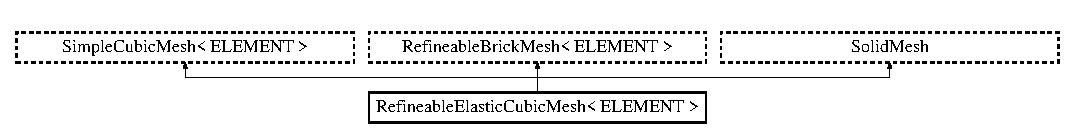
\includegraphics[height=1.419518cm]{classRefineableElasticCubicMesh}
\end{center}
\end{figure}
\subsection*{Public Member Functions}
\begin{DoxyCompactItemize}
\item 
\hyperlink{classRefineableElasticCubicMesh_a99c44a869363c33ed969a94256522b8c}{Refineable\+Elastic\+Cubic\+Mesh} (const unsigned \&nx, const unsigned \&ny, const unsigned \&nz, const double \&a, const double \&b, const double \&c, Time\+Stepper $\ast$time\+\_\+stepper\+\_\+pt=\&Mesh\+::\+Default\+\_\+\+Time\+Stepper)
\begin{DoxyCompactList}\small\item\em Constructor\+: \end{DoxyCompactList}\item 
virtual \hyperlink{classRefineableElasticCubicMesh_a2c0edb5ea4f205077285aced94af5767}{$\sim$\+Refineable\+Elastic\+Cubic\+Mesh} ()
\begin{DoxyCompactList}\small\item\em Empty Destructor. \end{DoxyCompactList}\end{DoxyCompactItemize}


\subsection{Detailed Description}
\subsubsection*{template$<$class E\+L\+E\+M\+E\+NT$>$\newline
class Refineable\+Elastic\+Cubic\+Mesh$<$ E\+L\+E\+M\+E\+N\+T $>$}

Simple cubic mesh upgraded to become a solid mesh. 

Definition at line 58 of file refineable\+\_\+simple\+\_\+shear.\+cc.



\subsection{Constructor \& Destructor Documentation}
\mbox{\Hypertarget{classRefineableElasticCubicMesh_a99c44a869363c33ed969a94256522b8c}\label{classRefineableElasticCubicMesh_a99c44a869363c33ed969a94256522b8c}} 
\index{Refineable\+Elastic\+Cubic\+Mesh@{Refineable\+Elastic\+Cubic\+Mesh}!Refineable\+Elastic\+Cubic\+Mesh@{Refineable\+Elastic\+Cubic\+Mesh}}
\index{Refineable\+Elastic\+Cubic\+Mesh@{Refineable\+Elastic\+Cubic\+Mesh}!Refineable\+Elastic\+Cubic\+Mesh@{Refineable\+Elastic\+Cubic\+Mesh}}
\subsubsection{\texorpdfstring{Refineable\+Elastic\+Cubic\+Mesh()}{RefineableElasticCubicMesh()}}
{\footnotesize\ttfamily template$<$class E\+L\+E\+M\+E\+NT$>$ \\
\hyperlink{classRefineableElasticCubicMesh}{Refineable\+Elastic\+Cubic\+Mesh}$<$ E\+L\+E\+M\+E\+NT $>$\+::\hyperlink{classRefineableElasticCubicMesh}{Refineable\+Elastic\+Cubic\+Mesh} (\begin{DoxyParamCaption}\item[{const unsigned \&}]{nx,  }\item[{const unsigned \&}]{ny,  }\item[{const unsigned \&}]{nz,  }\item[{const double \&}]{a,  }\item[{const double \&}]{b,  }\item[{const double \&}]{c,  }\item[{Time\+Stepper $\ast$}]{time\+\_\+stepper\+\_\+pt = {\ttfamily \&Mesh\+:\+:Default\+\_\+TimeStepper} }\end{DoxyParamCaption})\hspace{0.3cm}{\ttfamily [inline]}}



Constructor\+: 



Definition at line 66 of file refineable\+\_\+simple\+\_\+shear.\+cc.

\mbox{\Hypertarget{classRefineableElasticCubicMesh_a2c0edb5ea4f205077285aced94af5767}\label{classRefineableElasticCubicMesh_a2c0edb5ea4f205077285aced94af5767}} 
\index{Refineable\+Elastic\+Cubic\+Mesh@{Refineable\+Elastic\+Cubic\+Mesh}!````~Refineable\+Elastic\+Cubic\+Mesh@{$\sim$\+Refineable\+Elastic\+Cubic\+Mesh}}
\index{````~Refineable\+Elastic\+Cubic\+Mesh@{$\sim$\+Refineable\+Elastic\+Cubic\+Mesh}!Refineable\+Elastic\+Cubic\+Mesh@{Refineable\+Elastic\+Cubic\+Mesh}}
\subsubsection{\texorpdfstring{$\sim$\+Refineable\+Elastic\+Cubic\+Mesh()}{~RefineableElasticCubicMesh()}}
{\footnotesize\ttfamily template$<$class E\+L\+E\+M\+E\+NT$>$ \\
virtual \hyperlink{classRefineableElasticCubicMesh}{Refineable\+Elastic\+Cubic\+Mesh}$<$ E\+L\+E\+M\+E\+NT $>$\+::$\sim$\hyperlink{classRefineableElasticCubicMesh}{Refineable\+Elastic\+Cubic\+Mesh} (\begin{DoxyParamCaption}{ }\end{DoxyParamCaption})\hspace{0.3cm}{\ttfamily [inline]}, {\ttfamily [virtual]}}



Empty Destructor. 



Definition at line 82 of file refineable\+\_\+simple\+\_\+shear.\+cc.



The documentation for this class was generated from the following file\+:\begin{DoxyCompactItemize}
\item 
\hyperlink{refineable__simple__shear_8cc}{refineable\+\_\+simple\+\_\+shear.\+cc}\end{DoxyCompactItemize}

\hypertarget{classSimpleShearProblem}{}\section{Simple\+Shear\+Problem$<$ E\+L\+E\+M\+E\+NT $>$ Class Template Reference}
\label{classSimpleShearProblem}\index{Simple\+Shear\+Problem$<$ E\+L\+E\+M\+E\+N\+T $>$@{Simple\+Shear\+Problem$<$ E\+L\+E\+M\+E\+N\+T $>$}}


Boundary-\/driven elastic deformation of fish-\/shaped domain.  


Inheritance diagram for Simple\+Shear\+Problem$<$ E\+L\+E\+M\+E\+NT $>$\+:\begin{figure}[H]
\begin{center}
\leavevmode
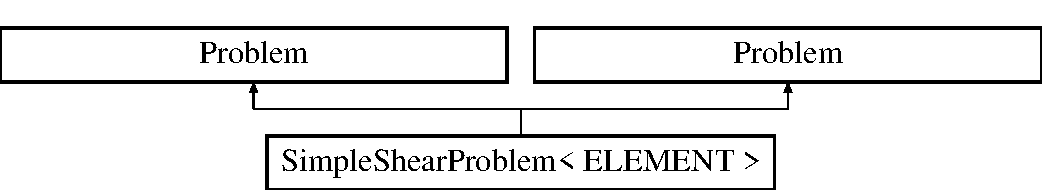
\includegraphics[height=2.000000cm]{classSimpleShearProblem}
\end{center}
\end{figure}
\subsection*{Public Member Functions}
\begin{DoxyCompactItemize}
\item 
\hyperlink{classSimpleShearProblem_ada0881781b3332f88362528be39613d2}{Simple\+Shear\+Problem} (const bool \&incompressible)
\begin{DoxyCompactList}\small\item\em Constructor\+: \end{DoxyCompactList}\item 
void \hyperlink{classSimpleShearProblem_ac1746a2634e310571d40d70719d509c0}{run} (const std\+::string \&dirname)
\begin{DoxyCompactList}\small\item\em Run simulation. \end{DoxyCompactList}\item 
\hyperlink{classRefineableElasticCubicMesh}{Refineable\+Elastic\+Cubic\+Mesh}$<$ E\+L\+E\+M\+E\+NT $>$ $\ast$ \hyperlink{classSimpleShearProblem_a2f13119c6c66305a6bde6945434a8f10}{mesh\+\_\+pt} ()
\begin{DoxyCompactList}\small\item\em Access function for the mesh. \end{DoxyCompactList}\item 
void \hyperlink{classSimpleShearProblem_a24c087d9ea194229930bcf9f889a048e}{doc\+\_\+solution} (Doc\+Info \&doc\+\_\+info)
\begin{DoxyCompactList}\small\item\em Doc the solution. \end{DoxyCompactList}\item 
void \hyperlink{classSimpleShearProblem_ab476064967687537e335dfd40d770dbc}{actions\+\_\+after\+\_\+newton\+\_\+solve} ()
\begin{DoxyCompactList}\small\item\em Update function (empty) \end{DoxyCompactList}\item 
void \hyperlink{classSimpleShearProblem_a17449af62f8025e2b03ddb922b47016d}{setup\+\_\+boundary\+\_\+conditions} ()
\item 
void \hyperlink{classSimpleShearProblem_a9b493680096cdbccb0cfa18b35787165}{actions\+\_\+after\+\_\+adapt} ()
\begin{DoxyCompactList}\small\item\em Need to pin the redundent solid pressures after adaptation. \end{DoxyCompactList}\item 
void \hyperlink{classSimpleShearProblem_a2c63e1a6c120da147b0c4ec9764e1510}{actions\+\_\+before\+\_\+newton\+\_\+solve} ()
\begin{DoxyCompactList}\small\item\em Update before solve\+: We\textquotesingle{}re dealing with a static problem so the nodal positions before the next solve merely serve as initial conditions. For meshes that are very strongly refined near the boundary, the update of the displacement boundary conditions (which only moves the Solid\+Nodes {\itshape on} the boundary), can lead to strongly distorted meshes. This can cause the Newton method to fail --$>$ the overall method is actually more robust if we use the nodal positions as determined by the Domain/\+Macro\+Element-\/ based mesh update as initial guesses. \end{DoxyCompactList}\item 
void \hyperlink{classSimpleShearProblem_a1069985934b36d269b4bc8cb3ba00902}{apply\+\_\+boundary\+\_\+conditions} ()
\begin{DoxyCompactList}\small\item\em Shear the top. \end{DoxyCompactList}\item 
\hyperlink{classSimpleShearProblem_ada0881781b3332f88362528be39613d2}{Simple\+Shear\+Problem} (const bool \&incompressible)
\begin{DoxyCompactList}\small\item\em Constructor\+: \end{DoxyCompactList}\item 
void \hyperlink{classSimpleShearProblem_ac1746a2634e310571d40d70719d509c0}{run} (const std\+::string \&dirname)
\begin{DoxyCompactList}\small\item\em Run simulation. \end{DoxyCompactList}\item 
\hyperlink{classElasticCubicMesh}{Elastic\+Cubic\+Mesh}$<$ E\+L\+E\+M\+E\+NT $>$ $\ast$ \hyperlink{classSimpleShearProblem_af1a0759d0c04c749b0f08fb7f936c0c6}{mesh\+\_\+pt} ()
\begin{DoxyCompactList}\small\item\em Access function for the mesh. \end{DoxyCompactList}\item 
void \hyperlink{classSimpleShearProblem_a24c087d9ea194229930bcf9f889a048e}{doc\+\_\+solution} (Doc\+Info \&doc\+\_\+info)
\begin{DoxyCompactList}\small\item\em Doc the solution. \end{DoxyCompactList}\item 
void \hyperlink{classSimpleShearProblem_ab476064967687537e335dfd40d770dbc}{actions\+\_\+after\+\_\+newton\+\_\+solve} ()
\begin{DoxyCompactList}\small\item\em Update function (empty) \end{DoxyCompactList}\item 
void \hyperlink{classSimpleShearProblem_a2c63e1a6c120da147b0c4ec9764e1510}{actions\+\_\+before\+\_\+newton\+\_\+solve} ()
\begin{DoxyCompactList}\small\item\em Update before solve\+: We\textquotesingle{}re dealing with a static problem so the nodal positions before the next solve merely serve as initial conditions. For meshes that are very strongly refined near the boundary, the update of the displacement boundary conditions (which only moves the Solid\+Nodes {\itshape on} the boundary), can lead to strongly distorted meshes. This can cause the Newton method to fail --$>$ the overall method is actually more robust if we use the nodal positions as determined by the Domain/\+Macro\+Element-\/ based mesh update as initial guesses. \end{DoxyCompactList}\item 
void \hyperlink{classSimpleShearProblem_a1069985934b36d269b4bc8cb3ba00902}{apply\+\_\+boundary\+\_\+conditions} ()
\begin{DoxyCompactList}\small\item\em Shear the top. \end{DoxyCompactList}\end{DoxyCompactItemize}
\subsection*{Private Member Functions}
\begin{DoxyCompactItemize}
\item 
void \hyperlink{classSimpleShearProblem_a3e5d5f57fc041531ee683f50395536f0}{set\+\_\+incompressible} (E\+L\+E\+M\+E\+NT $\ast$el\+\_\+pt, const bool \&incompressible)
\item 
void \hyperlink{classSimpleShearProblem_a3e5d5f57fc041531ee683f50395536f0}{set\+\_\+incompressible} (E\+L\+E\+M\+E\+NT $\ast$el\+\_\+pt, const bool \&incompressible)
\item 
{\footnotesize template$<$$>$ }\\void \hyperlink{classSimpleShearProblem_a064e94ff77e20bc81cd4ddbec58f26aa}{set\+\_\+incompressible} (Q\+P\+V\+D\+Element\+With\+Pressure$<$ 3 $>$ $\ast$el\+\_\+pt, const bool \&incompressible)
\item 
{\footnotesize template$<$$>$ }\\void \hyperlink{classSimpleShearProblem_a4f91c840813899e3977937e01e3bbb1e}{set\+\_\+incompressible} (Q\+P\+V\+D\+Element\+With\+Continuous\+Pressure$<$ 3 $>$ $\ast$el\+\_\+pt, const bool \&incompressible)
\item 
{\footnotesize template$<$$>$ }\\void \hyperlink{classSimpleShearProblem_af8ac5eb5a799de066ec2128905cd4ef6}{set\+\_\+incompressible} (Q\+P\+V\+D\+Element$<$ 3, 3 $>$ $\ast$el\+\_\+pt, const bool \&incompressible)
\item 
{\footnotesize template$<$$>$ }\\void \hyperlink{classSimpleShearProblem_a064e94ff77e20bc81cd4ddbec58f26aa}{set\+\_\+incompressible} (Q\+P\+V\+D\+Element\+With\+Pressure$<$ 3 $>$ $\ast$el\+\_\+pt, const bool \&incompressible)
\item 
{\footnotesize template$<$$>$ }\\void \hyperlink{classSimpleShearProblem_a4f91c840813899e3977937e01e3bbb1e}{set\+\_\+incompressible} (Q\+P\+V\+D\+Element\+With\+Continuous\+Pressure$<$ 3 $>$ $\ast$el\+\_\+pt, const bool \&incompressible)
\end{DoxyCompactItemize}
\subsection*{Private Attributes}
\begin{DoxyCompactItemize}
\item 
double \hyperlink{classSimpleShearProblem_a3844145c334e84c6ed94d803aeb1a337}{Shear}
\end{DoxyCompactItemize}


\subsection{Detailed Description}
\subsubsection*{template$<$class E\+L\+E\+M\+E\+NT$>$\newline
class Simple\+Shear\+Problem$<$ E\+L\+E\+M\+E\+N\+T $>$}

Boundary-\/driven elastic deformation of fish-\/shaped domain. 

Definition at line 141 of file refineable\+\_\+simple\+\_\+shear.\+cc.



\subsection{Constructor \& Destructor Documentation}
\mbox{\Hypertarget{classSimpleShearProblem_ada0881781b3332f88362528be39613d2}\label{classSimpleShearProblem_ada0881781b3332f88362528be39613d2}} 
\index{Simple\+Shear\+Problem@{Simple\+Shear\+Problem}!Simple\+Shear\+Problem@{Simple\+Shear\+Problem}}
\index{Simple\+Shear\+Problem@{Simple\+Shear\+Problem}!Simple\+Shear\+Problem@{Simple\+Shear\+Problem}}
\subsubsection{\texorpdfstring{Simple\+Shear\+Problem()}{SimpleShearProblem()}\hspace{0.1cm}{\footnotesize\ttfamily [1/2]}}
{\footnotesize\ttfamily template$<$class E\+L\+E\+M\+E\+NT $>$ \\
\hyperlink{classSimpleShearProblem}{Simple\+Shear\+Problem}$<$ E\+L\+E\+M\+E\+NT $>$\+::\hyperlink{classSimpleShearProblem}{Simple\+Shear\+Problem} (\begin{DoxyParamCaption}\item[{const bool \&}]{incompressible }\end{DoxyParamCaption})}



Constructor\+: 



Definition at line 244 of file refineable\+\_\+simple\+\_\+shear.\+cc.



References Global\+\_\+\+Physical\+\_\+\+Variables\+::\+Constitutive\+\_\+law\+\_\+pt, Simple\+Shear\+Problem$<$ E\+L\+E\+M\+E\+N\+T $>$\+::mesh\+\_\+pt(), Simple\+Shear\+Problem$<$ E\+L\+E\+M\+E\+N\+T $>$\+::set\+\_\+incompressible(), and Simple\+Shear\+Problem$<$ E\+L\+E\+M\+E\+N\+T $>$\+::setup\+\_\+boundary\+\_\+conditions().



Referenced by Simple\+Shear\+Problem$<$ E\+L\+E\+M\+E\+N\+T $>$\+::apply\+\_\+boundary\+\_\+conditions().

\mbox{\Hypertarget{classSimpleShearProblem_ada0881781b3332f88362528be39613d2}\label{classSimpleShearProblem_ada0881781b3332f88362528be39613d2}} 
\index{Simple\+Shear\+Problem@{Simple\+Shear\+Problem}!Simple\+Shear\+Problem@{Simple\+Shear\+Problem}}
\index{Simple\+Shear\+Problem@{Simple\+Shear\+Problem}!Simple\+Shear\+Problem@{Simple\+Shear\+Problem}}
\subsubsection{\texorpdfstring{Simple\+Shear\+Problem()}{SimpleShearProblem()}\hspace{0.1cm}{\footnotesize\ttfamily [2/2]}}
{\footnotesize\ttfamily template$<$class E\+L\+E\+M\+E\+NT$>$ \\
\hyperlink{classSimpleShearProblem}{Simple\+Shear\+Problem}$<$ E\+L\+E\+M\+E\+NT $>$\+::\hyperlink{classSimpleShearProblem}{Simple\+Shear\+Problem} (\begin{DoxyParamCaption}\item[{const bool \&}]{incompressible }\end{DoxyParamCaption})}



Constructor\+: 



\subsection{Member Function Documentation}
\mbox{\Hypertarget{classSimpleShearProblem_a9b493680096cdbccb0cfa18b35787165}\label{classSimpleShearProblem_a9b493680096cdbccb0cfa18b35787165}} 
\index{Simple\+Shear\+Problem@{Simple\+Shear\+Problem}!actions\+\_\+after\+\_\+adapt@{actions\+\_\+after\+\_\+adapt}}
\index{actions\+\_\+after\+\_\+adapt@{actions\+\_\+after\+\_\+adapt}!Simple\+Shear\+Problem@{Simple\+Shear\+Problem}}
\subsubsection{\texorpdfstring{actions\+\_\+after\+\_\+adapt()}{actions\_after\_adapt()}}
{\footnotesize\ttfamily template$<$class E\+L\+E\+M\+E\+NT$>$ \\
void \hyperlink{classSimpleShearProblem}{Simple\+Shear\+Problem}$<$ E\+L\+E\+M\+E\+NT $>$\+::actions\+\_\+after\+\_\+adapt (\begin{DoxyParamCaption}{ }\end{DoxyParamCaption})\hspace{0.3cm}{\ttfamily [inline]}}



Need to pin the redundent solid pressures after adaptation. 



Definition at line 194 of file refineable\+\_\+simple\+\_\+shear.\+cc.

\mbox{\Hypertarget{classSimpleShearProblem_ab476064967687537e335dfd40d770dbc}\label{classSimpleShearProblem_ab476064967687537e335dfd40d770dbc}} 
\index{Simple\+Shear\+Problem@{Simple\+Shear\+Problem}!actions\+\_\+after\+\_\+newton\+\_\+solve@{actions\+\_\+after\+\_\+newton\+\_\+solve}}
\index{actions\+\_\+after\+\_\+newton\+\_\+solve@{actions\+\_\+after\+\_\+newton\+\_\+solve}!Simple\+Shear\+Problem@{Simple\+Shear\+Problem}}
\subsubsection{\texorpdfstring{actions\+\_\+after\+\_\+newton\+\_\+solve()}{actions\_after\_newton\_solve()}\hspace{0.1cm}{\footnotesize\ttfamily [1/2]}}
{\footnotesize\ttfamily template$<$class E\+L\+E\+M\+E\+NT$>$ \\
void \hyperlink{classSimpleShearProblem}{Simple\+Shear\+Problem}$<$ E\+L\+E\+M\+E\+NT $>$\+::actions\+\_\+after\+\_\+newton\+\_\+solve (\begin{DoxyParamCaption}{ }\end{DoxyParamCaption})\hspace{0.3cm}{\ttfamily [inline]}}



Update function (empty) 



Definition at line 154 of file simple\+\_\+shear.\+cc.

\mbox{\Hypertarget{classSimpleShearProblem_ab476064967687537e335dfd40d770dbc}\label{classSimpleShearProblem_ab476064967687537e335dfd40d770dbc}} 
\index{Simple\+Shear\+Problem@{Simple\+Shear\+Problem}!actions\+\_\+after\+\_\+newton\+\_\+solve@{actions\+\_\+after\+\_\+newton\+\_\+solve}}
\index{actions\+\_\+after\+\_\+newton\+\_\+solve@{actions\+\_\+after\+\_\+newton\+\_\+solve}!Simple\+Shear\+Problem@{Simple\+Shear\+Problem}}
\subsubsection{\texorpdfstring{actions\+\_\+after\+\_\+newton\+\_\+solve()}{actions\_after\_newton\_solve()}\hspace{0.1cm}{\footnotesize\ttfamily [2/2]}}
{\footnotesize\ttfamily template$<$class E\+L\+E\+M\+E\+NT$>$ \\
void \hyperlink{classSimpleShearProblem}{Simple\+Shear\+Problem}$<$ E\+L\+E\+M\+E\+NT $>$\+::actions\+\_\+after\+\_\+newton\+\_\+solve (\begin{DoxyParamCaption}{ }\end{DoxyParamCaption})\hspace{0.3cm}{\ttfamily [inline]}}



Update function (empty) 



Definition at line 164 of file refineable\+\_\+simple\+\_\+shear.\+cc.

\mbox{\Hypertarget{classSimpleShearProblem_a2c63e1a6c120da147b0c4ec9764e1510}\label{classSimpleShearProblem_a2c63e1a6c120da147b0c4ec9764e1510}} 
\index{Simple\+Shear\+Problem@{Simple\+Shear\+Problem}!actions\+\_\+before\+\_\+newton\+\_\+solve@{actions\+\_\+before\+\_\+newton\+\_\+solve}}
\index{actions\+\_\+before\+\_\+newton\+\_\+solve@{actions\+\_\+before\+\_\+newton\+\_\+solve}!Simple\+Shear\+Problem@{Simple\+Shear\+Problem}}
\subsubsection{\texorpdfstring{actions\+\_\+before\+\_\+newton\+\_\+solve()}{actions\_before\_newton\_solve()}\hspace{0.1cm}{\footnotesize\ttfamily [1/2]}}
{\footnotesize\ttfamily template$<$class E\+L\+E\+M\+E\+NT$>$ \\
void \hyperlink{classSimpleShearProblem}{Simple\+Shear\+Problem}$<$ E\+L\+E\+M\+E\+NT $>$\+::actions\+\_\+before\+\_\+newton\+\_\+solve (\begin{DoxyParamCaption}{ }\end{DoxyParamCaption})\hspace{0.3cm}{\ttfamily [inline]}}



Update before solve\+: We\textquotesingle{}re dealing with a static problem so the nodal positions before the next solve merely serve as initial conditions. For meshes that are very strongly refined near the boundary, the update of the displacement boundary conditions (which only moves the Solid\+Nodes {\itshape on} the boundary), can lead to strongly distorted meshes. This can cause the Newton method to fail --$>$ the overall method is actually more robust if we use the nodal positions as determined by the Domain/\+Macro\+Element-\/ based mesh update as initial guesses. 



Definition at line 165 of file simple\+\_\+shear.\+cc.

\mbox{\Hypertarget{classSimpleShearProblem_a2c63e1a6c120da147b0c4ec9764e1510}\label{classSimpleShearProblem_a2c63e1a6c120da147b0c4ec9764e1510}} 
\index{Simple\+Shear\+Problem@{Simple\+Shear\+Problem}!actions\+\_\+before\+\_\+newton\+\_\+solve@{actions\+\_\+before\+\_\+newton\+\_\+solve}}
\index{actions\+\_\+before\+\_\+newton\+\_\+solve@{actions\+\_\+before\+\_\+newton\+\_\+solve}!Simple\+Shear\+Problem@{Simple\+Shear\+Problem}}
\subsubsection{\texorpdfstring{actions\+\_\+before\+\_\+newton\+\_\+solve()}{actions\_before\_newton\_solve()}\hspace{0.1cm}{\footnotesize\ttfamily [2/2]}}
{\footnotesize\ttfamily template$<$class E\+L\+E\+M\+E\+NT$>$ \\
void \hyperlink{classSimpleShearProblem}{Simple\+Shear\+Problem}$<$ E\+L\+E\+M\+E\+NT $>$\+::actions\+\_\+before\+\_\+newton\+\_\+solve (\begin{DoxyParamCaption}{ }\end{DoxyParamCaption})\hspace{0.3cm}{\ttfamily [inline]}}



Update before solve\+: We\textquotesingle{}re dealing with a static problem so the nodal positions before the next solve merely serve as initial conditions. For meshes that are very strongly refined near the boundary, the update of the displacement boundary conditions (which only moves the Solid\+Nodes {\itshape on} the boundary), can lead to strongly distorted meshes. This can cause the Newton method to fail --$>$ the overall method is actually more robust if we use the nodal positions as determined by the Domain/\+Macro\+Element-\/ based mesh update as initial guesses. 



Definition at line 216 of file refineable\+\_\+simple\+\_\+shear.\+cc.

\mbox{\Hypertarget{classSimpleShearProblem_a1069985934b36d269b4bc8cb3ba00902}\label{classSimpleShearProblem_a1069985934b36d269b4bc8cb3ba00902}} 
\index{Simple\+Shear\+Problem@{Simple\+Shear\+Problem}!apply\+\_\+boundary\+\_\+conditions@{apply\+\_\+boundary\+\_\+conditions}}
\index{apply\+\_\+boundary\+\_\+conditions@{apply\+\_\+boundary\+\_\+conditions}!Simple\+Shear\+Problem@{Simple\+Shear\+Problem}}
\subsubsection{\texorpdfstring{apply\+\_\+boundary\+\_\+conditions()}{apply\_boundary\_conditions()}\hspace{0.1cm}{\footnotesize\ttfamily [1/2]}}
{\footnotesize\ttfamily template$<$class E\+L\+E\+M\+E\+NT$>$ \\
void \hyperlink{classSimpleShearProblem}{Simple\+Shear\+Problem}$<$ E\+L\+E\+M\+E\+NT $>$\+::apply\+\_\+boundary\+\_\+conditions (\begin{DoxyParamCaption}{ }\end{DoxyParamCaption})\hspace{0.3cm}{\ttfamily [inline]}}



Shear the top. 



Definition at line 173 of file simple\+\_\+shear.\+cc.



References Global\+\_\+\+Physical\+\_\+\+Variables\+::\+Constitutive\+\_\+law\+\_\+pt, Simple\+Shear\+Problem$<$ E\+L\+E\+M\+E\+N\+T $>$\+::doc\+\_\+solution(), Global\+\_\+\+Physical\+\_\+\+Variables\+::\+Gravity, Simple\+Shear\+Problem$<$ E\+L\+E\+M\+E\+N\+T $>$\+::run(), and Simple\+Shear\+Problem$<$ E\+L\+E\+M\+E\+N\+T $>$\+::\+Simple\+Shear\+Problem().

\mbox{\Hypertarget{classSimpleShearProblem_a1069985934b36d269b4bc8cb3ba00902}\label{classSimpleShearProblem_a1069985934b36d269b4bc8cb3ba00902}} 
\index{Simple\+Shear\+Problem@{Simple\+Shear\+Problem}!apply\+\_\+boundary\+\_\+conditions@{apply\+\_\+boundary\+\_\+conditions}}
\index{apply\+\_\+boundary\+\_\+conditions@{apply\+\_\+boundary\+\_\+conditions}!Simple\+Shear\+Problem@{Simple\+Shear\+Problem}}
\subsubsection{\texorpdfstring{apply\+\_\+boundary\+\_\+conditions()}{apply\_boundary\_conditions()}\hspace{0.1cm}{\footnotesize\ttfamily [2/2]}}
{\footnotesize\ttfamily template$<$class E\+L\+E\+M\+E\+NT$>$ \\
void \hyperlink{classSimpleShearProblem}{Simple\+Shear\+Problem}$<$ E\+L\+E\+M\+E\+NT $>$\+::apply\+\_\+boundary\+\_\+conditions (\begin{DoxyParamCaption}{ }\end{DoxyParamCaption})\hspace{0.3cm}{\ttfamily [inline]}}



Shear the top. 



Definition at line 224 of file refineable\+\_\+simple\+\_\+shear.\+cc.

\mbox{\Hypertarget{classSimpleShearProblem_a24c087d9ea194229930bcf9f889a048e}\label{classSimpleShearProblem_a24c087d9ea194229930bcf9f889a048e}} 
\index{Simple\+Shear\+Problem@{Simple\+Shear\+Problem}!doc\+\_\+solution@{doc\+\_\+solution}}
\index{doc\+\_\+solution@{doc\+\_\+solution}!Simple\+Shear\+Problem@{Simple\+Shear\+Problem}}
\subsubsection{\texorpdfstring{doc\+\_\+solution()}{doc\_solution()}\hspace{0.1cm}{\footnotesize\ttfamily [1/2]}}
{\footnotesize\ttfamily template$<$class E\+L\+E\+M\+E\+NT$>$ \\
void \hyperlink{classSimpleShearProblem}{Simple\+Shear\+Problem}$<$ E\+L\+E\+M\+E\+NT $>$\+::doc\+\_\+solution (\begin{DoxyParamCaption}\item[{Doc\+Info \&}]{doc\+\_\+info }\end{DoxyParamCaption})}



Doc the solution. 

\mbox{\Hypertarget{classSimpleShearProblem_a24c087d9ea194229930bcf9f889a048e}\label{classSimpleShearProblem_a24c087d9ea194229930bcf9f889a048e}} 
\index{Simple\+Shear\+Problem@{Simple\+Shear\+Problem}!doc\+\_\+solution@{doc\+\_\+solution}}
\index{doc\+\_\+solution@{doc\+\_\+solution}!Simple\+Shear\+Problem@{Simple\+Shear\+Problem}}
\subsubsection{\texorpdfstring{doc\+\_\+solution()}{doc\_solution()}\hspace{0.1cm}{\footnotesize\ttfamily [2/2]}}
{\footnotesize\ttfamily template$<$class E\+L\+E\+M\+E\+NT $>$ \\
void \hyperlink{classSimpleShearProblem}{Simple\+Shear\+Problem}$<$ E\+L\+E\+M\+E\+NT $>$\+::doc\+\_\+solution (\begin{DoxyParamCaption}\item[{Doc\+Info \&}]{doc\+\_\+info }\end{DoxyParamCaption})}



Doc the solution. 



Definition at line 285 of file refineable\+\_\+simple\+\_\+shear.\+cc.



References Simple\+Shear\+Problem$<$ E\+L\+E\+M\+E\+N\+T $>$\+::mesh\+\_\+pt().



Referenced by Simple\+Shear\+Problem$<$ E\+L\+E\+M\+E\+N\+T $>$\+::apply\+\_\+boundary\+\_\+conditions(), and Simple\+Shear\+Problem$<$ E\+L\+E\+M\+E\+N\+T $>$\+::run().

\mbox{\Hypertarget{classSimpleShearProblem_af1a0759d0c04c749b0f08fb7f936c0c6}\label{classSimpleShearProblem_af1a0759d0c04c749b0f08fb7f936c0c6}} 
\index{Simple\+Shear\+Problem@{Simple\+Shear\+Problem}!mesh\+\_\+pt@{mesh\+\_\+pt}}
\index{mesh\+\_\+pt@{mesh\+\_\+pt}!Simple\+Shear\+Problem@{Simple\+Shear\+Problem}}
\subsubsection{\texorpdfstring{mesh\+\_\+pt()}{mesh\_pt()}\hspace{0.1cm}{\footnotesize\ttfamily [1/2]}}
{\footnotesize\ttfamily template$<$class E\+L\+E\+M\+E\+NT$>$ \\
\hyperlink{classElasticCubicMesh}{Elastic\+Cubic\+Mesh}$<$E\+L\+E\+M\+E\+NT$>$$\ast$ \hyperlink{classSimpleShearProblem}{Simple\+Shear\+Problem}$<$ E\+L\+E\+M\+E\+NT $>$\+::mesh\+\_\+pt (\begin{DoxyParamCaption}{ }\end{DoxyParamCaption})\hspace{0.3cm}{\ttfamily [inline]}}



Access function for the mesh. 



Definition at line 147 of file simple\+\_\+shear.\+cc.

\mbox{\Hypertarget{classSimpleShearProblem_a2f13119c6c66305a6bde6945434a8f10}\label{classSimpleShearProblem_a2f13119c6c66305a6bde6945434a8f10}} 
\index{Simple\+Shear\+Problem@{Simple\+Shear\+Problem}!mesh\+\_\+pt@{mesh\+\_\+pt}}
\index{mesh\+\_\+pt@{mesh\+\_\+pt}!Simple\+Shear\+Problem@{Simple\+Shear\+Problem}}
\subsubsection{\texorpdfstring{mesh\+\_\+pt()}{mesh\_pt()}\hspace{0.1cm}{\footnotesize\ttfamily [2/2]}}
{\footnotesize\ttfamily template$<$class E\+L\+E\+M\+E\+NT$>$ \\
\hyperlink{classRefineableElasticCubicMesh}{Refineable\+Elastic\+Cubic\+Mesh}$<$E\+L\+E\+M\+E\+NT$>$$\ast$ \hyperlink{classSimpleShearProblem}{Simple\+Shear\+Problem}$<$ E\+L\+E\+M\+E\+NT $>$\+::mesh\+\_\+pt (\begin{DoxyParamCaption}{ }\end{DoxyParamCaption})\hspace{0.3cm}{\ttfamily [inline]}}



Access function for the mesh. 



Definition at line 156 of file refineable\+\_\+simple\+\_\+shear.\+cc.



Referenced by Simple\+Shear\+Problem$<$ E\+L\+E\+M\+E\+N\+T $>$\+::doc\+\_\+solution(), and Simple\+Shear\+Problem$<$ E\+L\+E\+M\+E\+N\+T $>$\+::\+Simple\+Shear\+Problem().

\mbox{\Hypertarget{classSimpleShearProblem_ac1746a2634e310571d40d70719d509c0}\label{classSimpleShearProblem_ac1746a2634e310571d40d70719d509c0}} 
\index{Simple\+Shear\+Problem@{Simple\+Shear\+Problem}!run@{run}}
\index{run@{run}!Simple\+Shear\+Problem@{Simple\+Shear\+Problem}}
\subsubsection{\texorpdfstring{run()}{run()}\hspace{0.1cm}{\footnotesize\ttfamily [1/2]}}
{\footnotesize\ttfamily template$<$class E\+L\+E\+M\+E\+NT$>$ \\
void \hyperlink{classSimpleShearProblem}{Simple\+Shear\+Problem}$<$ E\+L\+E\+M\+E\+NT $>$\+::run (\begin{DoxyParamCaption}\item[{const std\+::string \&}]{dirname }\end{DoxyParamCaption})}



Run simulation. 

\mbox{\Hypertarget{classSimpleShearProblem_ac1746a2634e310571d40d70719d509c0}\label{classSimpleShearProblem_ac1746a2634e310571d40d70719d509c0}} 
\index{Simple\+Shear\+Problem@{Simple\+Shear\+Problem}!run@{run}}
\index{run@{run}!Simple\+Shear\+Problem@{Simple\+Shear\+Problem}}
\subsubsection{\texorpdfstring{run()}{run()}\hspace{0.1cm}{\footnotesize\ttfamily [2/2]}}
{\footnotesize\ttfamily template$<$class E\+L\+E\+M\+E\+NT $>$ \\
void \hyperlink{classSimpleShearProblem}{Simple\+Shear\+Problem}$<$ E\+L\+E\+M\+E\+NT $>$\+::run (\begin{DoxyParamCaption}\item[{const std\+::string \&}]{dirname }\end{DoxyParamCaption})}



Run simulation. 

Run the problem. 

Definition at line 339 of file refineable\+\_\+simple\+\_\+shear.\+cc.



References Simple\+Shear\+Problem$<$ E\+L\+E\+M\+E\+N\+T $>$\+::doc\+\_\+solution(), Global\+\_\+\+Physical\+\_\+\+Variables\+::\+Gravity, and Simple\+Shear\+Problem$<$ E\+L\+E\+M\+E\+N\+T $>$\+::\+Shear.



Referenced by Simple\+Shear\+Problem$<$ E\+L\+E\+M\+E\+N\+T $>$\+::apply\+\_\+boundary\+\_\+conditions(), and main().

\mbox{\Hypertarget{classSimpleShearProblem_a3e5d5f57fc041531ee683f50395536f0}\label{classSimpleShearProblem_a3e5d5f57fc041531ee683f50395536f0}} 
\index{Simple\+Shear\+Problem@{Simple\+Shear\+Problem}!set\+\_\+incompressible@{set\+\_\+incompressible}}
\index{set\+\_\+incompressible@{set\+\_\+incompressible}!Simple\+Shear\+Problem@{Simple\+Shear\+Problem}}
\subsubsection{\texorpdfstring{set\+\_\+incompressible()}{set\_incompressible()}\hspace{0.1cm}{\footnotesize\ttfamily [1/7]}}
{\footnotesize\ttfamily template$<$class E\+L\+E\+M\+E\+NT$>$ \\
void \hyperlink{classSimpleShearProblem}{Simple\+Shear\+Problem}$<$ E\+L\+E\+M\+E\+NT $>$\+::set\+\_\+incompressible (\begin{DoxyParamCaption}\item[{E\+L\+E\+M\+E\+NT $\ast$}]{el\+\_\+pt,  }\item[{const bool \&}]{incompressible }\end{DoxyParamCaption})\hspace{0.3cm}{\ttfamily [private]}}

\mbox{\Hypertarget{classSimpleShearProblem_a3e5d5f57fc041531ee683f50395536f0}\label{classSimpleShearProblem_a3e5d5f57fc041531ee683f50395536f0}} 
\index{Simple\+Shear\+Problem@{Simple\+Shear\+Problem}!set\+\_\+incompressible@{set\+\_\+incompressible}}
\index{set\+\_\+incompressible@{set\+\_\+incompressible}!Simple\+Shear\+Problem@{Simple\+Shear\+Problem}}
\subsubsection{\texorpdfstring{set\+\_\+incompressible()}{set\_incompressible()}\hspace{0.1cm}{\footnotesize\ttfamily [2/7]}}
{\footnotesize\ttfamily template$<$class E\+L\+E\+M\+E\+NT $>$ \\
void \hyperlink{classSimpleShearProblem}{Simple\+Shear\+Problem}$<$ E\+L\+E\+M\+E\+NT $>$\+::set\+\_\+incompressible (\begin{DoxyParamCaption}\item[{E\+L\+E\+M\+E\+NT $\ast$}]{el\+\_\+pt,  }\item[{const bool \&}]{incompressible }\end{DoxyParamCaption})\hspace{0.3cm}{\ttfamily [private]}}



Definition at line 383 of file refineable\+\_\+simple\+\_\+shear.\+cc.



Referenced by Simple\+Shear\+Problem$<$ E\+L\+E\+M\+E\+N\+T $>$\+::set\+\_\+incompressible(), and Simple\+Shear\+Problem$<$ E\+L\+E\+M\+E\+N\+T $>$\+::\+Simple\+Shear\+Problem().

\mbox{\Hypertarget{classSimpleShearProblem_af8ac5eb5a799de066ec2128905cd4ef6}\label{classSimpleShearProblem_af8ac5eb5a799de066ec2128905cd4ef6}} 
\index{Simple\+Shear\+Problem@{Simple\+Shear\+Problem}!set\+\_\+incompressible@{set\+\_\+incompressible}}
\index{set\+\_\+incompressible@{set\+\_\+incompressible}!Simple\+Shear\+Problem@{Simple\+Shear\+Problem}}
\subsubsection{\texorpdfstring{set\+\_\+incompressible()}{set\_incompressible()}\hspace{0.1cm}{\footnotesize\ttfamily [3/7]}}
{\footnotesize\ttfamily template$<$$>$ \\
void \hyperlink{classSimpleShearProblem}{Simple\+Shear\+Problem}$<$ Q\+P\+V\+D\+Element$<$ 3, 3 $>$ $>$\+::set\+\_\+incompressible (\begin{DoxyParamCaption}\item[{Q\+P\+V\+D\+Element$<$ 3, 3 $>$ $\ast$}]{el\+\_\+pt,  }\item[{const bool \&}]{incompressible }\end{DoxyParamCaption})\hspace{0.3cm}{\ttfamily [private]}}



Definition at line 341 of file simple\+\_\+shear.\+cc.

\mbox{\Hypertarget{classSimpleShearProblem_a064e94ff77e20bc81cd4ddbec58f26aa}\label{classSimpleShearProblem_a064e94ff77e20bc81cd4ddbec58f26aa}} 
\index{Simple\+Shear\+Problem@{Simple\+Shear\+Problem}!set\+\_\+incompressible@{set\+\_\+incompressible}}
\index{set\+\_\+incompressible@{set\+\_\+incompressible}!Simple\+Shear\+Problem@{Simple\+Shear\+Problem}}
\subsubsection{\texorpdfstring{set\+\_\+incompressible()}{set\_incompressible()}\hspace{0.1cm}{\footnotesize\ttfamily [4/7]}}
{\footnotesize\ttfamily template$<$$>$ \\
void \hyperlink{classSimpleShearProblem}{Simple\+Shear\+Problem}$<$ Q\+P\+V\+D\+Element\+With\+Pressure$<$ 3 $>$ $>$\+::set\+\_\+incompressible (\begin{DoxyParamCaption}\item[{Q\+P\+V\+D\+Element\+With\+Pressure$<$ 3 $>$ $\ast$}]{el\+\_\+pt,  }\item[{const bool \&}]{incompressible }\end{DoxyParamCaption})\hspace{0.3cm}{\ttfamily [private]}}



Definition at line 349 of file simple\+\_\+shear.\+cc.



References Simple\+Shear\+Problem$<$ E\+L\+E\+M\+E\+N\+T $>$\+::set\+\_\+incompressible().

\mbox{\Hypertarget{classSimpleShearProblem_a4f91c840813899e3977937e01e3bbb1e}\label{classSimpleShearProblem_a4f91c840813899e3977937e01e3bbb1e}} 
\index{Simple\+Shear\+Problem@{Simple\+Shear\+Problem}!set\+\_\+incompressible@{set\+\_\+incompressible}}
\index{set\+\_\+incompressible@{set\+\_\+incompressible}!Simple\+Shear\+Problem@{Simple\+Shear\+Problem}}
\subsubsection{\texorpdfstring{set\+\_\+incompressible()}{set\_incompressible()}\hspace{0.1cm}{\footnotesize\ttfamily [5/7]}}
{\footnotesize\ttfamily template$<$$>$ \\
void \hyperlink{classSimpleShearProblem}{Simple\+Shear\+Problem}$<$ Q\+P\+V\+D\+Element\+With\+Continuous\+Pressure$<$ 3 $>$ $>$\+::set\+\_\+incompressible (\begin{DoxyParamCaption}\item[{Q\+P\+V\+D\+Element\+With\+Continuous\+Pressure$<$ 3 $>$ $\ast$}]{el\+\_\+pt,  }\item[{const bool \&}]{incompressible }\end{DoxyParamCaption})\hspace{0.3cm}{\ttfamily [private]}}



Definition at line 358 of file simple\+\_\+shear.\+cc.



References Simple\+Shear\+Problem$<$ E\+L\+E\+M\+E\+N\+T $>$\+::set\+\_\+incompressible().

\mbox{\Hypertarget{classSimpleShearProblem_a064e94ff77e20bc81cd4ddbec58f26aa}\label{classSimpleShearProblem_a064e94ff77e20bc81cd4ddbec58f26aa}} 
\index{Simple\+Shear\+Problem@{Simple\+Shear\+Problem}!set\+\_\+incompressible@{set\+\_\+incompressible}}
\index{set\+\_\+incompressible@{set\+\_\+incompressible}!Simple\+Shear\+Problem@{Simple\+Shear\+Problem}}
\subsubsection{\texorpdfstring{set\+\_\+incompressible()}{set\_incompressible()}\hspace{0.1cm}{\footnotesize\ttfamily [6/7]}}
{\footnotesize\ttfamily template$<$$>$ \\
void \hyperlink{classSimpleShearProblem}{Simple\+Shear\+Problem}$<$ Q\+P\+V\+D\+Element\+With\+Pressure$<$ 3 $>$ $>$\+::set\+\_\+incompressible (\begin{DoxyParamCaption}\item[{Q\+P\+V\+D\+Element\+With\+Pressure$<$ 3 $>$ $\ast$}]{el\+\_\+pt,  }\item[{const bool \&}]{incompressible }\end{DoxyParamCaption})\hspace{0.3cm}{\ttfamily [private]}}



Definition at line 391 of file refineable\+\_\+simple\+\_\+shear.\+cc.



References Simple\+Shear\+Problem$<$ E\+L\+E\+M\+E\+N\+T $>$\+::set\+\_\+incompressible().

\mbox{\Hypertarget{classSimpleShearProblem_a4f91c840813899e3977937e01e3bbb1e}\label{classSimpleShearProblem_a4f91c840813899e3977937e01e3bbb1e}} 
\index{Simple\+Shear\+Problem@{Simple\+Shear\+Problem}!set\+\_\+incompressible@{set\+\_\+incompressible}}
\index{set\+\_\+incompressible@{set\+\_\+incompressible}!Simple\+Shear\+Problem@{Simple\+Shear\+Problem}}
\subsubsection{\texorpdfstring{set\+\_\+incompressible()}{set\_incompressible()}\hspace{0.1cm}{\footnotesize\ttfamily [7/7]}}
{\footnotesize\ttfamily template$<$$>$ \\
void \hyperlink{classSimpleShearProblem}{Simple\+Shear\+Problem}$<$ Q\+P\+V\+D\+Element\+With\+Continuous\+Pressure$<$ 3 $>$ $>$\+::set\+\_\+incompressible (\begin{DoxyParamCaption}\item[{Q\+P\+V\+D\+Element\+With\+Continuous\+Pressure$<$ 3 $>$ $\ast$}]{el\+\_\+pt,  }\item[{const bool \&}]{incompressible }\end{DoxyParamCaption})\hspace{0.3cm}{\ttfamily [private]}}



Definition at line 400 of file refineable\+\_\+simple\+\_\+shear.\+cc.

\mbox{\Hypertarget{classSimpleShearProblem_a17449af62f8025e2b03ddb922b47016d}\label{classSimpleShearProblem_a17449af62f8025e2b03ddb922b47016d}} 
\index{Simple\+Shear\+Problem@{Simple\+Shear\+Problem}!setup\+\_\+boundary\+\_\+conditions@{setup\+\_\+boundary\+\_\+conditions}}
\index{setup\+\_\+boundary\+\_\+conditions@{setup\+\_\+boundary\+\_\+conditions}!Simple\+Shear\+Problem@{Simple\+Shear\+Problem}}
\subsubsection{\texorpdfstring{setup\+\_\+boundary\+\_\+conditions()}{setup\_boundary\_conditions()}}
{\footnotesize\ttfamily template$<$class E\+L\+E\+M\+E\+NT$>$ \\
void \hyperlink{classSimpleShearProblem}{Simple\+Shear\+Problem}$<$ E\+L\+E\+M\+E\+NT $>$\+::setup\+\_\+boundary\+\_\+conditions (\begin{DoxyParamCaption}{ }\end{DoxyParamCaption})\hspace{0.3cm}{\ttfamily [inline]}}



Definition at line 166 of file refineable\+\_\+simple\+\_\+shear.\+cc.



Referenced by Simple\+Shear\+Problem$<$ E\+L\+E\+M\+E\+N\+T $>$\+::\+Simple\+Shear\+Problem().



\subsection{Member Data Documentation}
\mbox{\Hypertarget{classSimpleShearProblem_a3844145c334e84c6ed94d803aeb1a337}\label{classSimpleShearProblem_a3844145c334e84c6ed94d803aeb1a337}} 
\index{Simple\+Shear\+Problem@{Simple\+Shear\+Problem}!Shear@{Shear}}
\index{Shear@{Shear}!Simple\+Shear\+Problem@{Simple\+Shear\+Problem}}
\subsubsection{\texorpdfstring{Shear}{Shear}}
{\footnotesize\ttfamily template$<$class E\+L\+E\+M\+E\+NT$>$ \\
double \hyperlink{classSimpleShearProblem}{Simple\+Shear\+Problem}$<$ E\+L\+E\+M\+E\+NT $>$\+::Shear\hspace{0.3cm}{\ttfamily [private]}}



Definition at line 143 of file refineable\+\_\+simple\+\_\+shear.\+cc.



Referenced by Simple\+Shear\+Problem$<$ E\+L\+E\+M\+E\+N\+T $>$\+::run().



The documentation for this class was generated from the following files\+:\begin{DoxyCompactItemize}
\item 
\hyperlink{refineable__simple__shear_8cc}{refineable\+\_\+simple\+\_\+shear.\+cc}\item 
\hyperlink{simple__shear_8cc}{simple\+\_\+shear.\+cc}\end{DoxyCompactItemize}

\chapter{File Documentation}
\hypertarget{precompiled__mesh_8cc}{}\section{precompiled\+\_\+mesh.\+cc File Reference}
\label{precompiled__mesh_8cc}\index{precompiled\+\_\+mesh.\+cc@{precompiled\+\_\+mesh.\+cc}}

\hypertarget{refineable__simple__shear_8cc}{}\section{refineable\+\_\+simple\+\_\+shear.\+cc File Reference}
\label{refineable__simple__shear_8cc}\index{refineable\+\_\+simple\+\_\+shear.\+cc@{refineable\+\_\+simple\+\_\+shear.\+cc}}
\subsection*{Classes}
\begin{DoxyCompactItemize}
\item 
class \hyperlink{classRefineableElasticCubicMesh}{Refineable\+Elastic\+Cubic\+Mesh$<$ E\+L\+E\+M\+E\+N\+T $>$}
\begin{DoxyCompactList}\small\item\em Simple cubic mesh upgraded to become a solid mesh. \end{DoxyCompactList}\item 
class \hyperlink{classSimpleShearProblem}{Simple\+Shear\+Problem$<$ E\+L\+E\+M\+E\+N\+T $>$}
\begin{DoxyCompactList}\small\item\em Boundary-\/driven elastic deformation of fish-\/shaped domain. \end{DoxyCompactList}\end{DoxyCompactItemize}
\subsection*{Namespaces}
\begin{DoxyCompactItemize}
\item 
 \hyperlink{namespaceGlobal__Physical__Variables}{Global\+\_\+\+Physical\+\_\+\+Variables}
\begin{DoxyCompactList}\small\item\em Global variables. \end{DoxyCompactList}\end{DoxyCompactItemize}
\subsection*{Functions}
\begin{DoxyCompactItemize}
\item 
void \hyperlink{namespaceGlobal__Physical__Variables_a055c27a8d2375f73e74970a8ea1dee21}{Global\+\_\+\+Physical\+\_\+\+Variables\+::body\+\_\+force} (const Vector$<$ double $>$ \&xi, const double \&t, Vector$<$ double $>$ \&b)
\begin{DoxyCompactList}\small\item\em Body force vector\+: Vertically downwards with magnitude Gravity. \end{DoxyCompactList}\item 
int \hyperlink{refineable__simple__shear_8cc_ae66f6b31b5ad750f1fe042a706a4e3d4}{main} ()
\begin{DoxyCompactList}\small\item\em Driver for simple elastic problem. \end{DoxyCompactList}\end{DoxyCompactItemize}
\subsection*{Variables}
\begin{DoxyCompactItemize}
\item 
Strain\+Energy\+Function $\ast$ \hyperlink{namespaceGlobal__Physical__Variables_af6838abf46c7850f1ee0b3452d6d2498}{Global\+\_\+\+Physical\+\_\+\+Variables\+::\+Strain\+\_\+energy\+\_\+function\+\_\+pt}
\begin{DoxyCompactList}\small\item\em Pointer to strain energy function. \end{DoxyCompactList}\item 
Constitutive\+Law $\ast$ \hyperlink{namespaceGlobal__Physical__Variables_a5d5f19442938130d36ee7476ae25049c}{Global\+\_\+\+Physical\+\_\+\+Variables\+::\+Constitutive\+\_\+law\+\_\+pt}
\begin{DoxyCompactList}\small\item\em Pointer to constitutive law. \end{DoxyCompactList}\item 
double \hyperlink{namespaceGlobal__Physical__Variables_a09a019474b7405b35da2437f7779bc7e}{Global\+\_\+\+Physical\+\_\+\+Variables\+::E} =1.\+0
\begin{DoxyCompactList}\small\item\em Elastic modulus. \end{DoxyCompactList}\item 
double \hyperlink{namespaceGlobal__Physical__Variables_a3962c36313826b19f216f6bbbdd6a477}{Global\+\_\+\+Physical\+\_\+\+Variables\+::\+Nu} =0.\+3
\begin{DoxyCompactList}\small\item\em Poisson\textquotesingle{}s ratio. \end{DoxyCompactList}\item 
double \hyperlink{namespaceGlobal__Physical__Variables_a849754fa7155c1a31481674ce4845658}{Global\+\_\+\+Physical\+\_\+\+Variables\+::\+C1} =1.\+3
\begin{DoxyCompactList}\small\item\em \char`\"{}\+Mooney Rivlin\char`\"{} coefficient for generalised Mooney Rivlin law \end{DoxyCompactList}\item 
double \hyperlink{namespaceGlobal__Physical__Variables_a8b80d3e8d63b8d0a0ed435a2dd7fe2ad}{Global\+\_\+\+Physical\+\_\+\+Variables\+::\+Gravity} =0.\+0
\begin{DoxyCompactList}\small\item\em Body force. \end{DoxyCompactList}\end{DoxyCompactItemize}


\subsection{Function Documentation}
\mbox{\Hypertarget{refineable__simple__shear_8cc_ae66f6b31b5ad750f1fe042a706a4e3d4}\label{refineable__simple__shear_8cc_ae66f6b31b5ad750f1fe042a706a4e3d4}} 
\index{refineable\+\_\+simple\+\_\+shear.\+cc@{refineable\+\_\+simple\+\_\+shear.\+cc}!main@{main}}
\index{main@{main}!refineable\+\_\+simple\+\_\+shear.\+cc@{refineable\+\_\+simple\+\_\+shear.\+cc}}
\subsubsection{\texorpdfstring{main()}{main()}}
{\footnotesize\ttfamily int main (\begin{DoxyParamCaption}{ }\end{DoxyParamCaption})}



Driver for simple elastic problem. 



Definition at line 411 of file refineable\+\_\+simple\+\_\+shear.\+cc.



References Global\+\_\+\+Physical\+\_\+\+Variables\+::\+C1, Global\+\_\+\+Physical\+\_\+\+Variables\+::\+Constitutive\+\_\+law\+\_\+pt, Global\+\_\+\+Physical\+\_\+\+Variables\+::E, Global\+\_\+\+Physical\+\_\+\+Variables\+::\+Nu, Simple\+Shear\+Problem$<$ E\+L\+E\+M\+E\+N\+T $>$\+::run(), and Global\+\_\+\+Physical\+\_\+\+Variables\+::\+Strain\+\_\+energy\+\_\+function\+\_\+pt.


\hypertarget{simple__shear_8cc}{}\section{simple\+\_\+shear.\+cc File Reference}
\label{simple__shear_8cc}\index{simple\+\_\+shear.\+cc@{simple\+\_\+shear.\+cc}}
\subsection*{Classes}
\begin{DoxyCompactItemize}
\item 
class \hyperlink{classElasticCubicMesh}{Elastic\+Cubic\+Mesh$<$ E\+L\+E\+M\+E\+N\+T $>$}
\begin{DoxyCompactList}\small\item\em Simple cubic mesh upgraded to become a solid mesh. \end{DoxyCompactList}\item 
class \hyperlink{classSimpleShearProblem}{Simple\+Shear\+Problem$<$ E\+L\+E\+M\+E\+N\+T $>$}
\begin{DoxyCompactList}\small\item\em Boundary-\/driven elastic deformation of fish-\/shaped domain. \end{DoxyCompactList}\end{DoxyCompactItemize}
\subsection*{Namespaces}
\begin{DoxyCompactItemize}
\item 
 \hyperlink{namespaceGlobal__Physical__Variables}{Global\+\_\+\+Physical\+\_\+\+Variables}
\begin{DoxyCompactList}\small\item\em Global variables. \end{DoxyCompactList}\end{DoxyCompactItemize}
\subsection*{Functions}
\begin{DoxyCompactItemize}
\item 
void \hyperlink{namespaceGlobal__Physical__Variables_a055c27a8d2375f73e74970a8ea1dee21}{Global\+\_\+\+Physical\+\_\+\+Variables\+::body\+\_\+force} (const Vector$<$ double $>$ \&xi, const double \&t, Vector$<$ double $>$ \&b)
\begin{DoxyCompactList}\small\item\em Body force vector\+: Vertically downwards with magnitude Gravity. \end{DoxyCompactList}\item 
int \hyperlink{simple__shear_8cc_ae66f6b31b5ad750f1fe042a706a4e3d4}{main} ()
\begin{DoxyCompactList}\small\item\em Driver for simple elastic problem. \end{DoxyCompactList}\end{DoxyCompactItemize}


\subsection{Function Documentation}
\mbox{\Hypertarget{simple__shear_8cc_ae66f6b31b5ad750f1fe042a706a4e3d4}\label{simple__shear_8cc_ae66f6b31b5ad750f1fe042a706a4e3d4}} 
\index{simple\+\_\+shear.\+cc@{simple\+\_\+shear.\+cc}!main@{main}}
\index{main@{main}!simple\+\_\+shear.\+cc@{simple\+\_\+shear.\+cc}}
\subsubsection{\texorpdfstring{main()}{main()}}
{\footnotesize\ttfamily int main (\begin{DoxyParamCaption}{ }\end{DoxyParamCaption})}



Driver for simple elastic problem. 



Definition at line 369 of file simple\+\_\+shear.\+cc.



References Global\+\_\+\+Physical\+\_\+\+Variables\+::\+C1, Global\+\_\+\+Physical\+\_\+\+Variables\+::\+Constitutive\+\_\+law\+\_\+pt, Global\+\_\+\+Physical\+\_\+\+Variables\+::E, Global\+\_\+\+Physical\+\_\+\+Variables\+::\+Nu, Simple\+Shear\+Problem$<$ E\+L\+E\+M\+E\+N\+T $>$\+::run(), and Global\+\_\+\+Physical\+\_\+\+Variables\+::\+Strain\+\_\+energy\+\_\+function\+\_\+pt.


\hypertarget{simple__shear_8txt__doxygenified_8h}{}\section{simple\+\_\+shear.\+txt\+\_\+doxygenified.\+h File Reference}
\label{simple__shear_8txt__doxygenified_8h}\index{simple\+\_\+shear.\+txt\+\_\+doxygenified.\+h@{simple\+\_\+shear.\+txt\+\_\+doxygenified.\+h}}

%--- End generated contents ---

% Index
\backmatter
\newpage
\phantomsection
\clearemptydoublepage
\addcontentsline{toc}{chapter}{Index}
\printindex

